\documentclass[11pt]{article}
\usepackage{charsheet}
\usepackage{multicol}
\usepackage{amsmath}
\usetikzlibrary{fit}
%\usepackage{amsmath}
\colorlet{grayed out}{white!70!black}

\newcommand\scrm[1]{\textrm{\textsc{#1}}}

\newcommand\bigstrut{\vrule width 0pt height 16pt depth 0pt }

\usepackage{pgfkeys}

% Incomplete character support



\newdimen\textmargin % amount subtracted from each side to get `text width`
\textmargin=8pt

\newdimen\mynodedistance
\mynodedistance=7pt

\tikzset{%
  minimum label sep=6pt,
  every label node part/.style={
     text width=,
     font=\sffamily\footnotesize,
  },
  widecolumn/.style={
    labeled decorated stub rectangle,
    text width=134mm-2\textmargin,
    inner xsep=8pt,
    align=justify,
    font={\rightskip=0pt plus 2em},
    inner ysep=6pt,
    outer xsep=0pt, % x placement is happening by hand
    draw, line width=1.2pt,
    stub radius=2.3mm,
  },
  narrowcolumn/.style={
    widecolumn,
    text width=36mm-2\textmargin,
  },
  initiative/.style={
    labeled decorated clipped rectangle,
%    minimum width=\hpwidth/3-10pt,
    draw, line width=1.2pt,
    fill=white,
%    yseparated,
    outer xsep=3pt,
    minimum height=17mm,
  },
  dnd hit dice/.style={
    dnd max hp,
%    labeled decorated clipped rectangle,
%    yseparated,
%    minimum width=\hpwidth/2-5pt,
    minimum height=18mm,
    font=\footnotesize,
  }
}

  

\newcommand\fboxzero[1]{{\fboxsep=0pt \fbox{#1}}}


\begin{document}




%\input{stats}

\noindent
\begin{charsheet}
  \tikzset{node distance=\mynodedistance}

\node [anchor=south west] (merman) at (0,0) {
   \vbox{
    \vspace*{15mm}
   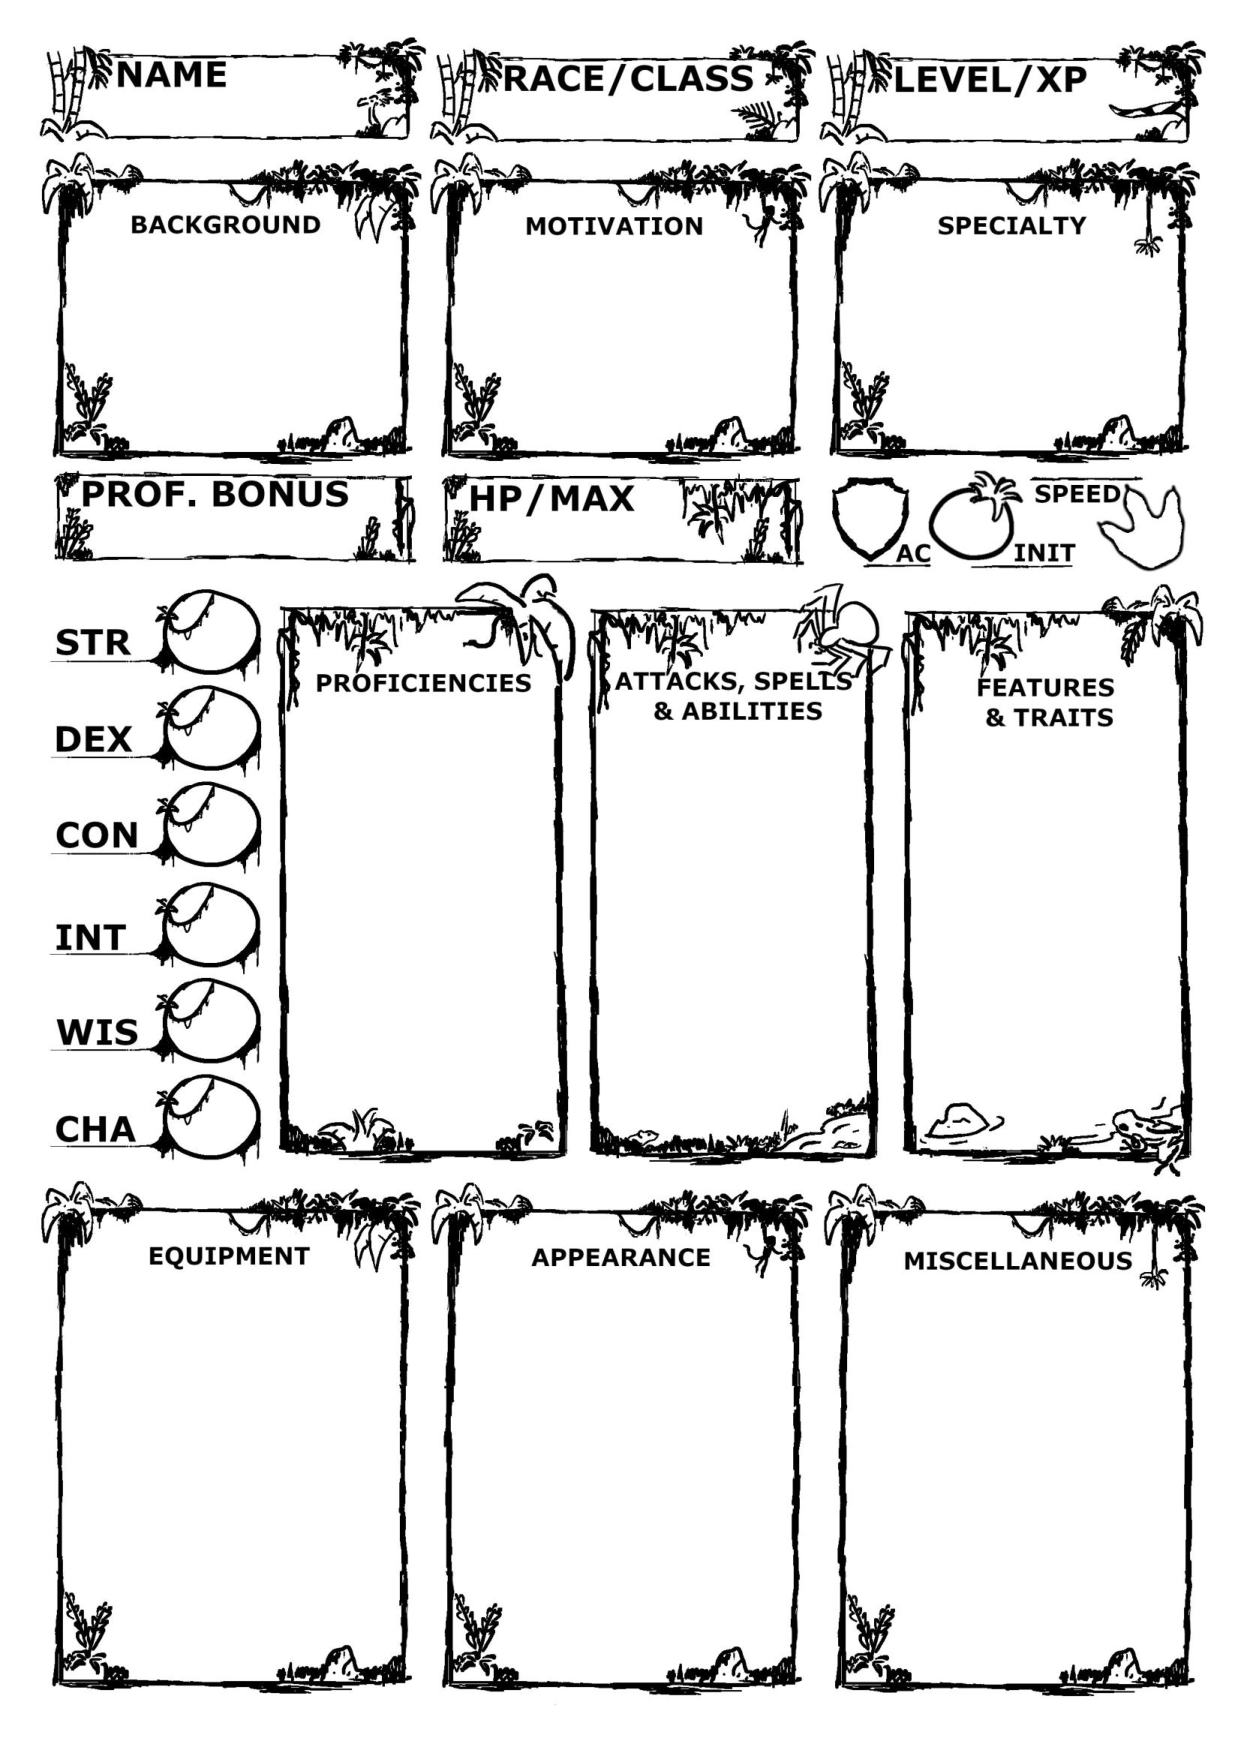
\includegraphics[height=\paperheight]{angry-custom-1.pdf}
    \vspace*{-15mm}
   }
};

% Grid overlay: thin line every 1mm, heavy every 10mm, labels every 10mm.
% Grid is anchored to the image's SW corner so labels align with gridlines.
\begin{scope}
  \clip (merman.south west) rectangle (merman.north east);
  \draw[blue!40, line width=0.1pt]
    (merman.south west) grid[step=1] (merman.north east);
  \draw[blue, line width=0.8pt]
    (merman.south west) grid[step=10] (merman.north east);
  \foreach \x in {0,10,...,300} {
    \node[anchor=south west, font=\tiny\sffamily\bfseries,
          text=blue, inner sep=1pt]
      at ([xshift=\x mm]merman.south west) {\x};
  }
  \foreach \y in {10,20,...,300} {
    \node[anchor=south west, font=\tiny\sffamily\bfseries,
          text=blue, inner sep=1pt]
      at ([yshift=\y mm]merman.south west) {\y};
  }
\end{scope}


%%%%      \begingroup\sffamily
%%%%    
%%%%      \newcommand\namestrut{\vrule width 0pt depth 1pt\relax}
%%%%    
%%%%      \path ($(splash.south west)+(88mm,18.75mm)$) coordinate  (class field sw);
%%%%      \path ($(splash.south west)+(88mm,9.7mm)$) coordinate  (race field sw);
%%%%      \path ($(splash.south west)+(48mm,16mm)$) coordinate  (charname center);
%%%%      \path ($(splash.south west)+(40mm,24mm)$) coordinate  (pregen left);
%%%%     
%%%%    
%%%%      \ifDNDfalse{PREGENERATED}%
%%%%        {\node [fill=splashgray,width=42mm,height=5mm,anchor=south west,at=(pregen left)] {};}
%%%%        {}
%%%%    
%%%%    
%%%%      \node [fill=splashfield,width=97mm,height=6mm,anchor=south west,at=(class field sw)] {};
%%%%      \node [fill=splashfield,width=97mm,height=6mm,anchor=south west,at=(race field sw)] {};
%%%%    
%%%%      \path (class field sw) +(0mm,0.6mm) coordinate (class sw);
%%%%      \path (race field sw) +(0mm,0.6mm) coordinate (race sw);
%%%%    
%%%%      \writesplash[at=(class sw)]{34mm}{CLASS + LEVEL}
%%%%      \writesplash[right of base=1mm of CLASS + LEVEL]{28mm}{BACKGROUND}
%%%%      \writesplash[right of base=1mm of BACKGROUND]{34mm}{PLAYER NAME}
%%%%    
%%%%      \writesplash[at=(race sw)]{34mm}{RACE}
%%%%      \writesplash[right of base=1mm of RACE]{34mm}{ALIGNMENT}
%%%%      \writesplash[right of base=1mm of ALIGNMENT]{34mm}{EXPERIENCE POINTS}
%%%%    
%%%%      \ifDNDdefined{CHARACTER NAME}
%%%%    {\node[at=(charname center),font={\rmfamily\LARGE\itshape},anchor=center]
%%%%          {\getDND{CHARACTER NAME}\ifDNDnonempty{AGE}{ \Large (\getDND{AGE})}{}}
%%%%          ;
%%%%        }
%%%%        {}
%%%%    
%%%%    \Large
%%%%    
%%%%        \setnodeheight\sectionheight[dnd max hp]
%%%%        \setnodeheight\tmpheight[dnd hit dice]
%%%%        \advance\sectionheight by \tmpheight
%%%%        \advance\sectionheight by 3\mynodedistance
%%%%        \def\hdwidth{20mm}
%%%%        \def\chpwidth{72mm}
%%%%        \setlength\sectionwidth{\hdwidth+\chpwidth+3\mynodedistance}
%%%%    
%%%%          \node (hpbackground) 
%%%%            [outer sep=0pt,stub rectangle,fill=hit points background,below right corner=of splash,
%%%%             width=\sectionwidth, height=\sectionheight] 
%%%%           { };
%%%%    
%%%%          \node (hitdice)
%%%%                 [dnd hit dice,labeled decorated clipped rectangle,width=\hdwidth,inside south east corner=of hpbackground,
%%%%                 font=\Large] 
%%%%             {\nodepart{label}HIT DICE\nodepart{ctext}
%%%%                \vrule height 8mm width 0pt\getDND*{HIT DICE}}
%%%%             ;
%%%%    
%%%%         \ifDNDdefined{LEVEL}{
%%%%             \node [at=(hitdice.north),anchor=north] 
%%%%                  {\expandafter\stackslots\expandafter{\rawgetDND{LEVEL}+1}};
%%%%         }{}
%%%%    
%%%%          \node (curhp)
%%%%                [dnd hit dice,labeled decorated clipped rectangle,fill=white,width=\chpwidth,left=of hitdice,
%%%%                 ] 
%%%%             { \nodepart{label}CURRENT HIT POINTS }
%%%%             ;
%%%%    
%%%%          \node [dnd max hp,above left corner=of curhp] 
%%%%             (maxhp)
%%%%             {\nodepart{label}MAX HP\nodepart{ctext}\getDND*{MAX HP}}
%%%%             ;
%%%%    
%%%%          \node (initiative)
%%%%                [dnd max hp,right=of maxhp] 
%%%%             {\nodepart{label}INITIATIVE\nodepart{ctext}\getDND*{INITIATIVE}}
%%%%             ;
%%%%    
%%%%    %\node [draw,above=of initiative] % {\slotsliteral7};
%%%%    %              {\expandafter\stackslots\expandafter{\rawgetDND{LEVEL}+1}};
%%%%    
%%%%    
%%%%          \node (speed)
%%%%                [dnd max hp,right=of initiative] 
%%%%             {\nodepart{label}SPEED\nodepart{ctext}\getDND*{SPEED}}
%%%%             ;
%%%%    
%%%%    
%%%%           \node (ac) [dnd max hp,shield,inner shield,draw,ultra thick,right=of speed,width=15mm,
%%%%                       font=\Large,
%%%%                ]
%%%%          {\getDND*{ARMOR CLASS}}
%%%%          ;
%%%%          \node [above=3pt of ac.south] {\tinystacklabel{ARMOR}{CLASS}}
%%%%          ;
%%%%    
%%%%    
%%%%      \endgroup
%%%%    
%%%%     \node (attacks) [widecolumn,fill=attacks,below right corner=of hpbackground]
%%%%        {\nodepart{label}ATTACKS\nodepart{text}
%%%%        \centering
%%%%        \useDNDfont*{ATTACKS}
%%%%        \noindent
%%%%        \begin{attackstab}
%%%%        \gdef\notesheader{\cline{2-4}}%
%%%%        \gdef\notesheader{}%
%%%%        \gdef\attacknote#1#2{}%  Just don't
%%%%        \getDND{ATTACKS}%
%%%%        \end{attackstab}%
%%%%        \renewenvironment{attacknotes}{\small\begin{multicols}{2}}{\end{multicols}}%
%%%%        \renewcommand\attacknote[2]{%
%%%%          {{\raggedright\smallskip\noindent\emph{#1:} {#2}\hangindent=1.5em \hangafter=1\par}}%
%%%%        }%
%%%%        \DNDattacknotes
%%%%    }
%%%%      ;
%%%%    
%%%%    
%%%%    
%%%%    
%%%%    % \node (attacks) at (hpbackground.south west) {A};
%%%%    
%%%%    \ifDNDdefined{MAGIC}
%%%%    {
%%%%      \node (magic) [widecolumn,below=of attacks,fill=magic]
%%%%        {\nodepart{label}MAGIC\nodepart{text}
%%%%         \featurespostspace=0pt
%%%%         \centering
%%%%         \useDNDfont{MAGIC}
%%%%         \newcommand\spellslevellabel[2]{\multicolumn2{@{}l@{}}{\spellslevel[#2]{#1}}\\}%
%%%%         \begin{featurestab}
%%%%         \rawgetDND{MAGIC}
%%%%         \end{featurestab}
%%%%        }
%%%%      ;
%%%%    }
%%%%    {\path (attacks.south east) coordinate (magic);} % anchor is to east
%%%%    
%%%%    \ifDNDdefined{FEATURES}{
%%%%      \ifDNDdefined{MAGIC}
%%%%         {\def\where{anchor=south east,at=(current bounding box.south -| magic.east)}
%%%%          \featurespostspace=3pt
%%%%         }
%%%%         {\def\where{below right corner=of attacks}%
%%%%          \advance\featurespostspace by 2pt
%%%%         }%
%%%%       \expandafter\node\expandafter[\where,widecolumn,fill=features] 
%%%%         (features)
%%%%         {\nodepart{label}FEATURES\nodepart{text}
%%%%          \let\described=\feature
%%%%          \let\describedColored=\featureColored
%%%%          \useDNDfont*{FEATURES}
%%%%          \begin{featurestab}
%%%%          \getDND{FEATURES}
%%%%          \end{featurestab}
%%%%         };
%%%%    }{}
%%%%    
%%%%    \setnodewidth\sectionwidth[statbox]
%%%%    \setnodeheight\sectionheight[statbox]
%%%%    \node (stats background) 
%%%%          [stub rectangle,stub radius=6pt,fill=stats,width=\sectionwidth+2\mynodedistance+0.5\savingshieldwidth,
%%%%           height=6\sectionheight+7\mynodedistance+24mm+5mm, % % * 4mm, ellipses
%%%%           below left corner=of splash
%%%%          ] { };
%%%%    
%%%%    \newcommand\nextstatloc{inside north west corner=5mm and \mynodedistance of stats background}
%%%%    
%%%%    \dndstat{STRENGTH}{STR}
%%%%    \dndstat{DEXTERITY}{DEX}
%%%%    \dndstat{CONSTITUTION}{CON}
%%%%    \dndstat{INTELLIGENCE}{INT}
%%%%    \dndstat{WISDOM}{WIS}
%%%%    \dndstat{CHARISMA}{CHA}
%%%%    
%%%%    \path (stats background.north -| attacks.west) ++(-\mynodedistance,0)
%%%%       coordinate (prof ne);
%%%%    
%%%%    
%%%%    % \draw [red,thick] (prof circle west) circle [radius=3pt];
%%%%    
%%%%    
%%%%    
%%%%    % slots OK here
%%%%    
%%%%    \setnodeheight\tmpheight[coin]
%%%%    \setlength\sectionheight{4\tmpheight+5\mynodedistance}
%%%%       % make room for four coin boxes
%%%%    
%%%%    \ifDNDdefined{EQUIPMENT}{%
%%%%       \setnodewidth\sectionwidth[widecolumn]
%%%%       \ifDNDdefined{MAGIC}
%%%%            {\def\where{left of lower corner=of features}
%%%%             \setdeltax\sectionwidth{magic.west}{stats background.west}
%%%%             \advance\sectionwidth by -\mynodedistance
%%%%            }
%%%%            {\def\where{below right corner=of features}}
%%%%       \multicolsep=0pt
%%%%       \expandafter\node\expandafter
%%%%           [\where,widecolumn,fill=equipment,decorated labeled clipped rectangle,
%%%%            minimum height=\sectionheight,
%%%%            text width=\sectionwidth-2\textmargin,
%%%%           ]
%%%%           (equipment)
%%%%         {
%%%%           \nodepart{label}EQUIPMENT\nodepart{text}
%%%%    %       \medskip
%%%%           \noindent
%%%%           \hspace*{21mm-5pt}%  leave room for coins on left
%%%%           \begin{minipage}{\hsize-21mm-5pt}
%%%%           \ifnum\rawgetDND{EQUIPMENT COLS}=1
%%%%           \else
%%%%              \begin{multicols}{\rawgetDND{EQUIPMENT COLS}}
%%%%           \fi
%%%%           \small
%%%%           \useDNDfont{EQUIPMENT}%
%%%%            \begin{eqlist}%
%%%%           \ifDNDnonempty{EQUIPMENT}
%%%%              {\getDND{EQUIPMENT}}
%%%%              {\item (Placeholder: Equipment will go here.)}%
%%%%           \end{eqlist}
%%%%           \ifnum\rawgetDND{EQUIPMENT COLS}=1
%%%%           \else
%%%%             \end{multicols}
%%%%           \fi
%%%%           \end{minipage}%
%%%%         }
%%%%        ;
%%%%    }{
%%%%      \node (equipment) [draw=none,fill=none,left of lower corner=of features] {};
%%%%    }
%%%%    
%%%%    \path (equipment.north west) +(3mm,-\mynodedistance) coordinate (coin top left);
%%%%    
%%%%    \coin{cp}{Cu}{\color{grayed out}\getDND*{CP}}
%%%%    \coin{sp}{Ag}{\color{grayed out}\getDND*{SP}}
%%%%    \coin{gp}{Au}{\color{grayed out}\getDND*{GP}}
%%%%    \coin{pp}{Pt}{\color{grayed out}\getDND*{PP}}
%%%%      
%%%%    \setdeltax\sectionwidth{attacks.west}{stats background.east}
%%%%    \node (proficiency bonus)
%%%%          [proficiencies,decorated stub rectangle,
%%%%           width=\sectionwidth-2\mynodedistance-5mm+2mm, % room for circle
%%%%           height=8mm,
%%%%           anchor=north east,
%%%%           at=(prof ne),
%%%%          ]
%%%%       {}
%%%%       ;
%%%%    \path (stats background.east) ++(\mynodedistance,0) ++(-2.5pt,0) coordinate (prof circle west);
%%%%    \node (proficiency circle) [anchor=west,proficiencies,circle,
%%%%           width=10mm,height=10mm,line width=1.5pt,draw]
%%%%           at (prof circle west |- proficiency bonus.center)
%%%%          {\large\textsf{+\arabic{proficiency bonus}}};
%%%%    
%%%%    \draw [line width=0.5pt] (proficiency circle) circle [radius=4.2mm];
%%%%    
%%%%    % center the text in the visible space
%%%%    \setdeltax\tmpwidth{proficiency bonus.east}{proficiency circle.east}
%%%%    
%%%%    \path (proficiency circle.east) ++(0.5\tmpwidth,0)
%%%%          ++(-1.1mm,0) % for inset
%%%%          node {\tiny\textsf{PROFICIENCY BONUS}}
%%%%          ;
%%%%    
%%%%    % proficiencies bottom should be stats background bottom or equipment
%%%%    % top, whatever is higher
%%%%    
%%%%    
%%%%      \setdeltay\tmpheight{stats background.south}{equipment.north}
%%%%      \advance\tmpheight by -\mynodedistance % allows space above equipment.north
%%%%      \ifdim\tmpheight>0pt
%%%%        \setdeltay\sectionheight{proficiency bonus.south}{stats background.south}
%%%%        \advance\sectionheight by -\mynodedistance
%%%%      \else
%%%%        \setdeltay\sectionheight{proficiency bonus.south}{equipment.north}
%%%%        \advance\sectionheight by -2\mynodedistance
%%%%      \fi
%%%%    
%%%%    
%%%%      \node (proficiencies)
%%%%          [widecolumn,fill=proficiencies,
%%%%           text width=\sectionwidth-2\mynodedistance-2\textmargin,
%%%%           height=\sectionheight,
%%%%           below right corner=of proficiency bonus,
%%%%          ]
%%%%       {\nodepart{label}PROFICIENCIES\nodepart{text}
%%%%         \vspace*{-2pt} % too much inner ysep at the top
%%%%         \useDNDfont*{PROFICIENCIES}
%%%%         \newif\ifprofs
%%%%         \profsfalse
%%%%         \whenDNDnonempty{PROFICIENCIES}\profstrue
%%%%         \whenDNDnonempty{SECONDARY PROFICIENCIES}\profstrue
%%%%         \begin{proflist}
%%%%         \getDND*{PROFICIENCIES}
%%%%         \whenDNDnonempty{PROFICIENCIES}{%
%%%%             \whenDNDnonempty{SECONDARY PROFICIENCIES}{\profskip}}
%%%%         \getDND*{SECONDARY PROFICIENCIES}
%%%%         \relax
%%%%         \ifprofs\else \item (No proficiencies listed.)\fi
%%%%         \end{proflist}
%%%%       }
%%%%     ;
%%%%    
%%%%    
%%%%    
%%%%    
%%%%    %\node (motivation) [below=of proficiencies] 
%%%%    %  {\parbox{36mm}{\Large\centering\textit{\getDND*{MOTIVATION}}}}
%%%%    %  ;
%%%%    
%%%%    \node (motivations) [above=4.45mm of BACKGROUND.north] 
%%%%      {\whenDNDnonempty{MOTIVATION}{\Large\textit{Motivation: \getDND*{MOTIVATION}}}}
%%%%      ;
%%%%    
%%%%    % choose the first two nonempty from this list to display as upper and lower
%%%%    \firsttwoDNDnonempty{\upperdndlabel}{\upperdndcontents}{\lowerdndlabel}{\lowerdndcontents}{SORCERY POINTS,SENSES,SPELL DC,PASSIVE PERCEPTION}
%%%%    
%%%%    \def\sp{SORCERY POINTS}
%%%%    \ifx\upperdndlabel\sp
%%%%      \edef\upperdndcontents{\noexpand\stackslots{\rawgetDND{SORCERY POINTS}}}%
%%%%    \fi
%%%%    
%%%%    \def\se{SENSES}
%%%%    \ifx\upperdndlabel\se
%%%%      \def\upperdndcontents{\parbox{20mm}{\centering\rmfamily\small\textit{\getDND{SENSES}}}}%
%%%%    \fi
%%%%    
%%%%    %\show\pp
%%%%    %\show\upperdndlabel
%%%%    
%%%%    \setdeltax\tmpwidth{hpbackground.west}{proficiencies.east}
%%%%    \path (proficiencies.east) ++(0.5\tmpwidth,0) coordinate (special center);
%%%%    
%%%%      \node (upper val)
%%%%             [dnd max hp,width=28mm] 
%%%%          at (special center |- maxhp.center)
%%%%             {\nodepart{label}
%%%%              \ifDNDfont{\upperdndlabel}{\useDNDfont{\upperdndlabel}}{}%
%%%%              \hbox to 0pt{\hss\upperdndlabel\hss}%
%%%%              \nodepart{ctext}
%%%%              \Large\textsf{\upperdndcontents}}
%%%%             ;
%%%%    
%%%%    \ifx\lowerdndlabel\empty\else
%%%%    
%%%%       \node (lower val)
%%%%          [dnd max hp,width=28mm]
%%%%          at (special center |- curhp.center)
%%%%          {\nodepart{label}
%%%%           \ifDNDfont{\lowerdndlabel}{\useDNDfont{\lowerdndlabel}}{}%
%%%%           \hbox to 0pt{\hss\lowerdndlabel\hss}%
%%%%           \nodepart{ctext}
%%%%           \Large\textsf{\lowerdndcontents}
%%%%          }
%%%%          ;
%%%%    
%%%%    \fi
%%%%    
%%%%    
%%%%    %\node [draw,above=of features] {\parbox{4in}{7 slots: minimum \minrows{7} rows\par \stackslots7\par\hbox{\slotsliteral3}}};


\end{charsheet}

\whenDNDtrue{VALIDATION ERRORS}
{
\section{Validation errors}
\begin{itemize}
\getDND{VALIDATION ERRORS}
\end{itemize}
}

\end{document}
